\documentclass{scrreprt}
\usepackage{listings}
\usepackage{underscore}
\usepackage[bookmarks=true]{hyperref}
\usepackage[utf8]{inputenc}
\usepackage[english]{babel}

\usepackage{tcolorbox}
\usepackage{hyperref}

\hypersetup{
    bookmarks=false,    % show bookmarks bar?
    pdftitle={FP PROJECT REPORT},    % title
    pdfauthor={Saptarishi Dhanuka},                     % author
    pdfsubject={TeX and LaTeX},                        % subject of the document
    pdfkeywords={TeX, LaTeX, graphics, images}, % list of keywords
    colorlinks=true,       % false: boxed links; true: colored links
    linkcolor=blue,       % color of internal links
    citecolor=black,       % color of links to bibliography
    filecolor=black,        % color of file links
    urlcolor=purple,        % color of external links
    linktoc=page            % only page is linked
}%
\def\myversion{1.0 }
\date{}
%\title
\usepackage{hyperref}
\begin{document}

\begin{flushright}
    \rule{16cm}{5pt}\vskip1cm
    \begin{bfseries}
        \Huge{FUNCTIONAL PROGRAMMING \\ CS-IS-2010-1 \\ MIDTERM EVALUATION \\ PROJECT REPORT}\\
        \vspace{1.9cm}
        Haskell Web Scraper\\
        \vspace{1.9cm}
        Saptarishi Dhanuka\\
        \vspace{1.9cm}
        Ashoka University\\
    \end{bfseries}
\end{flushright}

\tableofcontents



\chapter{Problem Statement and Requirements}
\begin{tcolorbox}[colback=white,colframe=gray,title={Assigned Project Statement}]
    Develop a scraper using Haskell to extract text and code snippets separately.
    \begin{enumerate}
        \item \textbf{Input}: Scrape the text and code snippets from the given text \href{https://eli.thegreenplace.net/2018/type-erasure-and-reification/}{source}
        \item \textbf{Output}: A Word document containing the text and \texttt{.txt} file containing the code.
        \item \textbf{Method}: Write the algorithm to scrape (you can use the \texttt{tagsoup} library) and all the input-output facilities using Haskell. Do not use any other language.
    \end{enumerate}
\end{tcolorbox}

% in the design section can give the basic structure of the HTML page

\section{Problem Description}
The given web page is made of text and code snippets, which we need to scrape and extract separately into a \texttt{.docx} file containing the text portions and a \texttt{.txt} file which has the code snippets. \\ For this, we need to fetch the given web page, parse and analyze its HTML structure to identify the HTML tags of the code snippets and the tags of the rest of the text, so that we can effectively separate them into different documents.


\section{Requirements}

\begin{enumerate}
    \item The scraper shall be written entirely in Haskell
    \item The scraper shall get all text of the given page and write it into a \texttt{.docx} file.
    \item The scraper shall get all the code snippets of the given page and write it into a \texttt{.txt} file.
\end{enumerate}



% \begin{enumerate}
%     \item \textbf{Functional}
%     \begin{enumerate}
%         \item The scraper will be written entirely in Haskell
%         \item The scraper will accurately get all text of the given page and write it in a formatted manner into the \texttt{.txt} file. It will preserve the order and structure of the text on the page
%         \item The scraper will accurately get the code snippets of the given page and write it in ordered manner into a \texttt{.docx} file.
%     \end{enumerate}
    
%     \item \textbf{Non-functional}
%     \begin{enumerate}
%         \item The scraper will gracefully handle any errors that occur during it's running
%     \end{enumerate}
        
% \end{enumerate}



\chapter{Specifications}


\begin{enumerate}
    \item The scraper will use Haskell HTTP libraries for fetching the HTML content of the given web page.
    \item The scraper will separate the code snippets from the rest of the textual content using an algorithm that utilizes the \texttt{tagsoup} library to parse the HTML content, along with other standard libraries for string and text handling.
    \item The scraper will write the text into a Word document and the code snippets into a \texttt{.txt} file mainly using the \texttt{tagsoup} and \texttt{pandoc} libraries, along with some standard Haskell libraries.
    \item The \texttt{.txt} file will be formatted such that the code snippets are visibly delimited for readability purposes.
    \item The \texttt{.docx} file will be formatted in a manner similar to the original web page in terms of demarcating headings, footnotes and the order of the text. 
\end{enumerate}




% \begin{enumerate}
%     \item \textbf{Limitations} % should limitations go here or later on cause it's seeming out of place here
%     % this can go in the design and architecture part or in the specs part
%     \begin{enumerate}
%         \item Since the HTML structure of different web pages can vary, it is not necessary that this particular scraper will work for all web pages. It is designed specifically for the given page and may work for some other pages. But no generalisation can be made about the correctness of its text and code extraction for other pages.
%         \item Moreover, it will not necessarily work for web pages with malformed HTML or different structure.
%         \item It is not designed to be robust to design changes, which is in line with the \href{https://hackage.haskell.org/package/tagsoup-0.6/src/tagsoup.htm#:~:text=Rule%202%3A%0ADo%20not%20be%20robust%20to%20design%20changes%2C%20do%20not%20even%20consider%20the%20possibility%20when%20writing%20the%20code.}{rule} stated on the \texttt{tagsoup} library's documentation example. If the site's HTML structure changes, for instance if the code snippets change from being enclosed in \texttt{<pre>} tags to \texttt{<code>} tags, then the scraper will not be able to separate out the code from the text and extract them accurately.
%     \end{enumerate}
% \end{enumerate}






\chapter{Design and Architecture}
% need to put functions into Lib and main stuff in main
% mention directory structure here along with basic ideas of the functions and code what it's doing


\section{High-Level Architecture}

% insert image here
\begin{figure}[h]
    \centering
    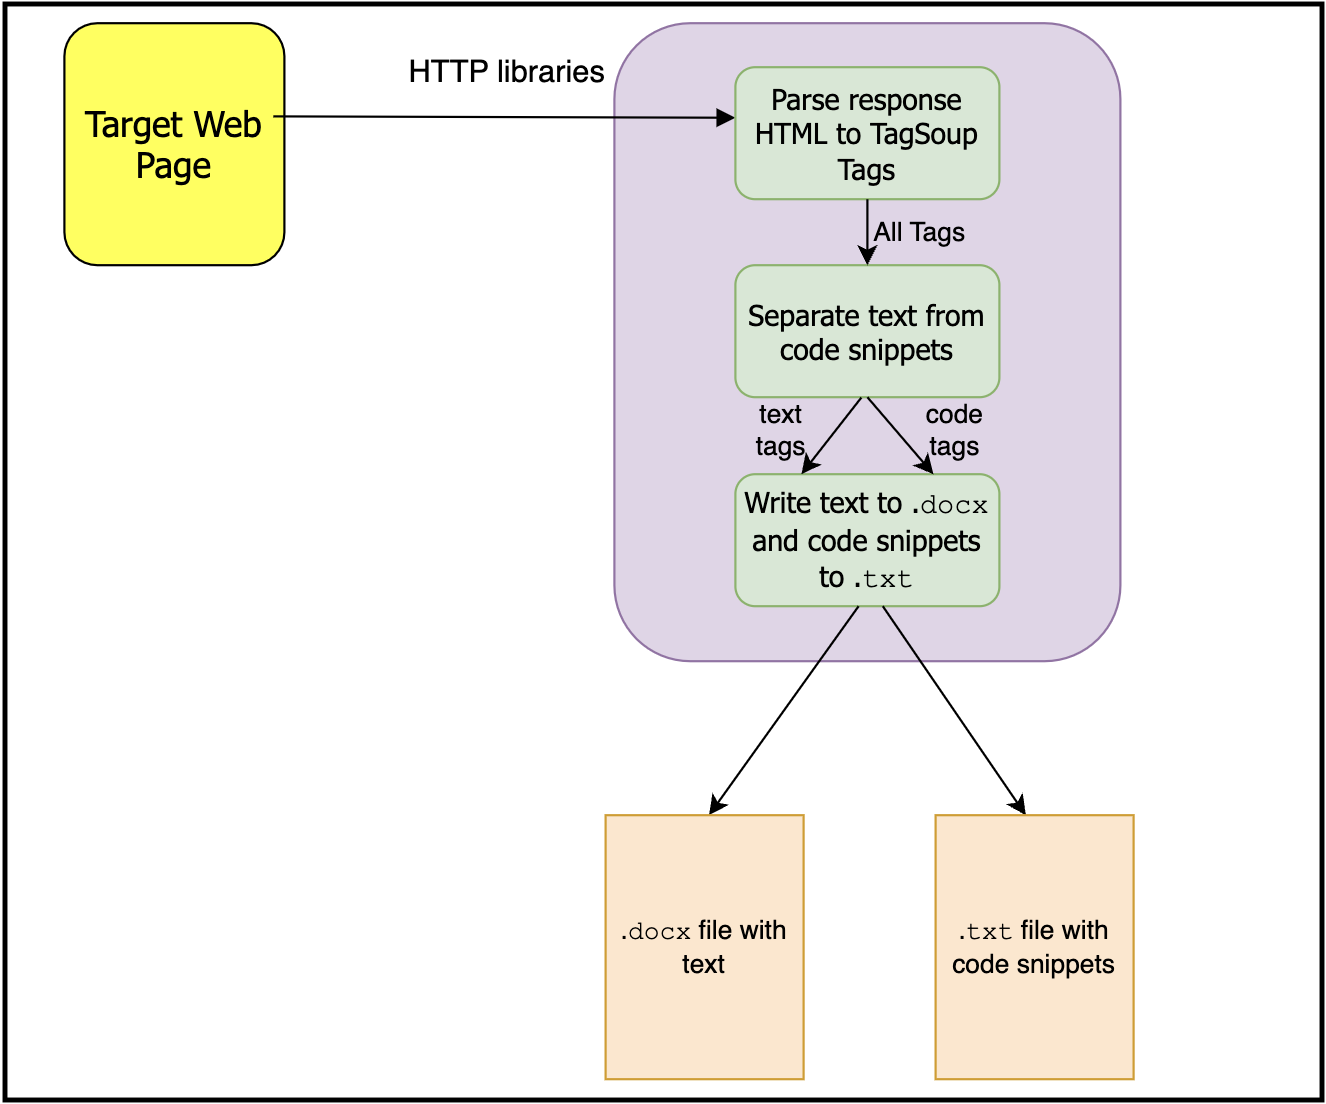
\includegraphics[width=1.0\textwidth]{figures/high-arch.png}
    \caption{High-Level Architecture}
    \label{fig:high-level-arch}
\end{figure}

The \textbf{high-level architecture} consists of the following:
\begin{enumerate}
    \item Functionality for getting the target web page using HTTP libraries.
    \item Parsing the response obtained from the HTTP libraries into Tags from the \texttt{tagsoup} library.
    \item Separating the text from the code snippets using the descriptions of each Tag from the above Tags
    \item Extracting the visible content from the text tags and writing them into a \texttt{.docx} file
    \item Extracting the visible content from the code tags and writing them into a \texttt{.txt} file
\end{enumerate}



\section{High-Level Design}


\begin{figure}[h]
    \centering
    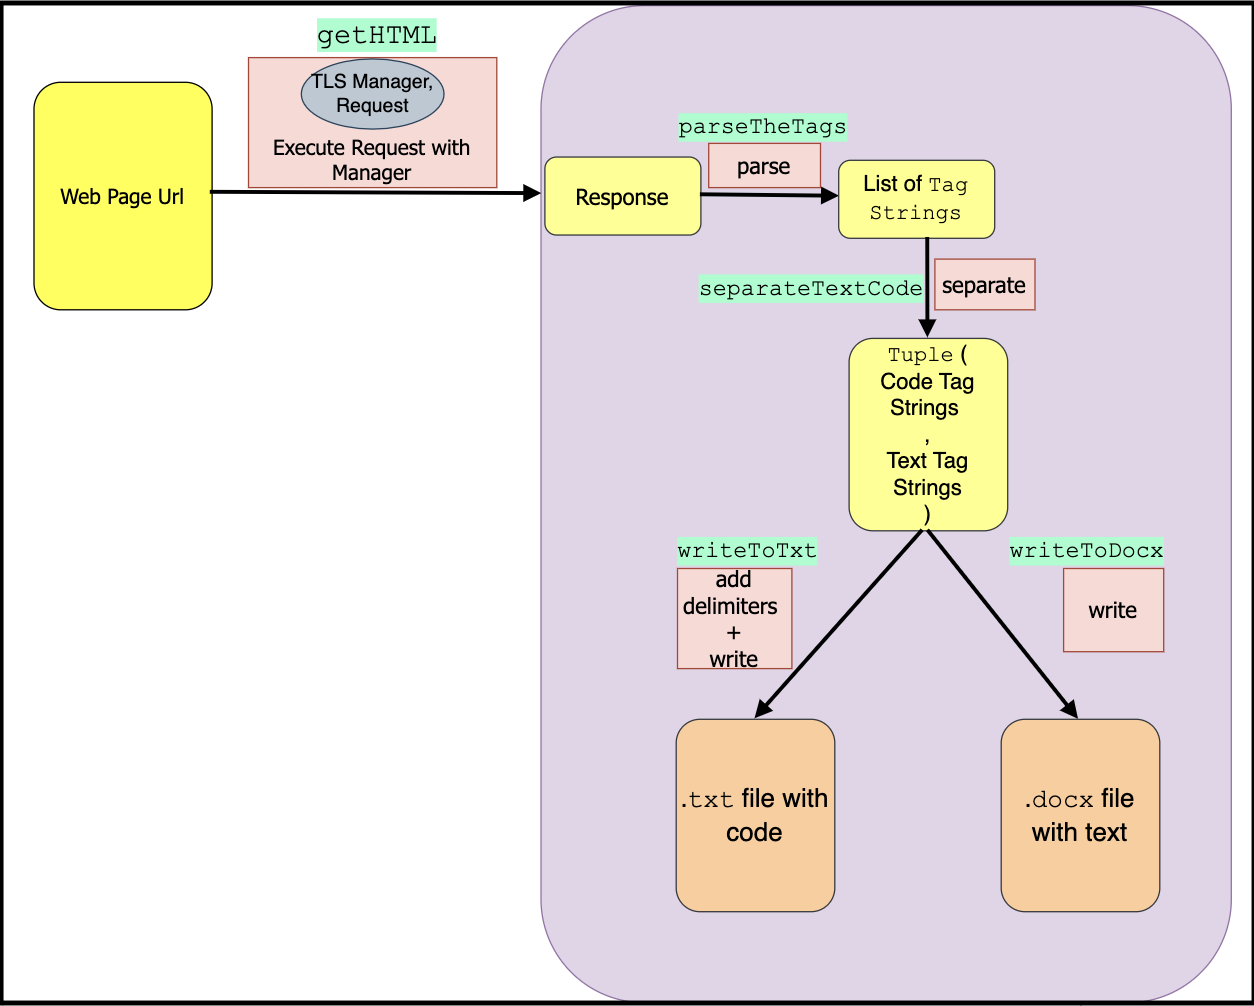
\includegraphics[width=1.0\textwidth]{figures/high-design.png}
    \caption{High-Level Design with functions in highlighted in cyan}
    \label{fig:high-level-design}
\end{figure}

The \textbf{high-level design} which implements the above architecture consists of the following:
\begin{enumerate}
    \item A TLS manager for handling HTTPS requests, since the given URL is prefixed with \texttt{https}
    \item Parsing the url into a request
    \item Executing the request with the TLS manager
    \item Get the body i.e. the HTML content from the response received after executing the request
    \item Parse the HTML into a list of Tag Strings according to the \texttt{tagsoup} library
    \item Separate the Tags corresponding to the code from the Tags corresponding to the textual content. By inspecting the HTML, we can see that the code snippets are within \texttt{<pre>} tags, so we need to separate everything enclosed within these tags from the rest of the HTML content. We also remove images. 
    \item Insert delimiters between each \texttt{<pre>} tag for formatting purposes. 
    \item Convert the list of Tag Strings corresponding to the code and to the text each back into an HTML-formatted string, which we then convert into a \texttt{pandoc} document as intermediate representation
    \item Convert the pandocs into another intermediate string-like format which can then be written into the respective \texttt{.docx} and \texttt{.txt} files
\end{enumerate}


\section{Low-Level design}
The core low-level design that has been abstracted away from the above design and architecture is mentioned below


\begin{enumerate}
    % should i analyse this algorithm??
    \item \textbf{Separation of text from code} \\ 
    \\ \textbf{Idea:} Create a boolean list corresponding to every element of the list of Tag Strings. A boolean list element will be True if a Tag is a \texttt{<pre>} tag or within a \texttt{<pre>} tag, or if it's an \texttt{<img>} tag. Then zip the boolean list with the original list and divide into two lists based on the boolean value, then extract the Tag elements from each separate list.\\
    \\ \textbf{Steps:}
    \begin{verbatim}
        1. Create list of booleans which have elements to be True if the 
        corresponding Tags from the Tag String list are <pre> tags
        2. Make all those tags in between open and closing <pre> tags also true
        3. Create a tuple which combines each Tag with their 
        corresponding Boolean value, then select those Tags who have a True value. This is our list of code Tags
        4. Create list of booleans which have elements to be True if the 
        corresponding Tags from the Tag String list are <img> tags
        5. Create overall boolean list whose elements are true if the
         corresponding tag is within a <pre> tag or is an <img> tag
        6. Create a tuple which combines each Tag with their corresponding 
        Boolean value, then select those Tags who have a False value. 
        This is our list of text Tags
    \end{verbatim}

    \item \textbf{Writing to .txt file} \\ 
    \textbf{Steps:}
    \begin{verbatim}
        1. Insert delimiter after every closing <pre> tag
        2. Convert the Tag Strings back to HTML-formatted string
        3. Convert into pandoc as intermediate representation, and 
        then further into Text with writePlain
        4. Write this Text into the .txt file
    \end{verbatim} 

    \item \textbf{Writing to .docx file} \\ 
    \textbf{Steps:}
    \begin{verbatim}
        2. Convert the Tag Strings back to HTML-formatted string
        3. Convert into pandoc as intermediate representation, and 
        then further into ByteString with writeDocx
        4. Write this ByteString into the .docx file
    \end{verbatim} 
    
    
\end{enumerate}











\chapter {Tools and Languages}
% tech stack
% need to be clear on cabal stack and haskell and stuff


\section{Languages}

Only Haskell was used for the project as mentioned in the problem statement

\section{Tools}

\begin{enumerate}
    \item The Glasgow Haskell Compiler (GHC) is used for compilation.
    \item \href{https://docs.haskellstack.org/en/stable/}{Stack} is used as the build tool. This manages installing project dependencies, building and running the project and testing the project.
    \item \textbf{Libraries}:
    \begin{enumerate}
        \item \texttt{Network.HTTP.Client.TLS} was chosen for handling HTTPS connections in order to use the \texttt{newTlsManager} function
        \item \texttt{Network.HTTP.Client} was chosen for parsing the url into a request, executing the request with the manager, and getting the body from the response. The functions used were \texttt{parseRequest, httpLbs, responseBody} respectively.
        \item \texttt{Tagsoup} was used to parse the HTML into a list of Tag Strings, and then also to convert the separated Tag Strings back into an HTML-formatted string . It was also used in a helper function that inserted a delimiter between the code snippets. The functions used were \texttt{parseTags, isTagOpenName, isTagCloseName, renderTags}, along with the \texttt{TagText} constructor and \texttt{Tag} for \texttt{Tag String}.
        \item \texttt{Pandoc} was used to read the HTML-formatted strings for both the code and the text into intermediate Pandoc representation. Then it was used to write the content into another intermediate string-like representation, which in turn was written into the final files with a standard library. The functions used were \texttt{readHtml, writePlain, writeDocx, runIO}.
        \item \texttt{Data.ByteString.Lazy.Char8} was used to convert the ByteString obtained from the response body into a string for further processing. The function used was \texttt{unpack}
        \item \texttt{Data.ByteString.Lazy} was used to write the ByteString obtained from the \texttt{writeDocx} function from \texttt{pandoc}, into the final \texttt{.docx} file. The function used was \texttt{writeFile}
        \item \texttt{Data.Text.Conversions} was used to convert the separated HTML strings into the \texttt{Text} type defined under \texttt{Data.Text}, so that it could be converted into intermediate pandoc representation by \texttt{readHtml}. The function used was \texttt{convertText}.
        \item \texttt{Data.Text} was used in order to use the \texttt{Text} type
        \item \texttt{Data.Text.IO} was used to write the Text obtained from the \texttt{writePlain} function from \texttt{pandoc}, into the final \texttt{.txt} file. The function used was \texttt{writeFile}
        \item The standard \texttt{Prelude} was used for various operations.
    \end{enumerate} 
\end{enumerate}






\chapter{Test Plan}
% test individual functions 
% for the midterm eval at the end if have time (need to) then can write one big test 

\section{Tools to be used for Testing}



\section{Test Suite Outline}

\begin{enumerate}
    \item \textbf{Unit Testing}: The following functions can be tested 
    \begin{enumerate}
        \item \texttt{getHTML : }
        \begin{enumerate}
            \item Test if the function returns the correct HTML for various URLs by using sample inputs and outputs.
            \item Test if the function gracefully handles invalid URLs with error handling.
            \item Test if the function handles network errors and HTTPS errors with error handling.
        \end{enumerate}

        \item \texttt{parseTheTags : }
        \begin{enumerate}
            \item Test if the function returns the correct list of Tag Strings for various HTML content.
            \item Test if the function handles malformed HTML and erroneous inputs with error handling.
            \item 
        \end{enumerate}

        \item \texttt{fillTrue : }
        \begin{enumerate}
            \item Test if the function correctly fills in True values for all elements within any two matching pair of True values corresponding to \texttt{<pre>} tags.
            \item Test if the function handles edge cases with empty lists or single element lists.
        \end{enumerate}

        \item \texttt{insertNewLines : }
        \begin{enumerate}
            \item Test if the function correctly adds the delimiter before every closing \texttt{<pre>} tag.
            \item Test if the function handles cases where there are no \texttt{<pre>} tags, or the Tag String is malformed 
        \end{enumerate}

        \item \texttt{separateTextCode : }
        \begin{enumerate}
            \item Test if the function correctly returns a tuple of two lists where one list has the Tag Strings corresponding to all the content enclosed within \texttt{<pre>} tags, and that the other list has all the other elements, excluding images.
            \item Test edge cases of no \texttt{<pre>} tags, nested \texttt{<pre>} tags
        \end{enumerate}

        \item \texttt{writeToTxt : }
        While File I/O cannot be unit-tested in the traditional sense, we can still manually test the file outputs.
        \begin{enumerate}
            \item Test if the function correctly writes the content of the input Tag String with delimters to the \texttt{.txt} file using sample input output
        \end{enumerate}

        \item \texttt{writeToDocx : }
        While File I/O cannot be unit-tested in the traditional sense, we can still manually test the file outputs.
        \begin{enumerate}
            \item Test if the function correctly writes the content of the input Tag String to the \texttt{.docx} file using sample input output
        \end{enumerate}




    \end{enumerate}
    \item 
\end{enumerate}






\chapter{Prototype Implementation Details}
% this can give a broad overview of what the prototype can and cannot do. What the input and output of the prototype look like etc.




\chapter{Plan for Completion}
% will test. will do error handling. formal verification and validation stuff and maybe make more robust for other urls also idk. Getting better performance



















\end{document}